\documentclass{article}
 
\usepackage[T2A]{fontenc}
\usepackage[utf8]{inputenc}
\usepackage[bulgarian]{babel}
\usepackage{cite}
\usepackage{graphicx}
\usepackage{amsmath}
\usepackage{amsfonts}
\usepackage{float}
\usepackage{amssymb}

\graphicspath{{images/}}

\title{Изследване на скалируемостта на Wa-Tor симулацията при cтатична декомпозиция на домейна}

\author{Иван-Асен Веселинов Чакъров \\
	ФН: 81837, Курс: 3, Група: 1}
\date{Юли 2021}


\begin{document}

\maketitle

\section{Увод}
Wa-Tor симулацията~\cite{wator} е класически проблем при паралелното програмиране.
Накратко проблемът е симулирането на идеализиран двумерен свят с формата на тор.
Светът има два вида обитатели - херинги, които играят ролята на плячка и акули, които ловят херингите
Подробните правилата за симулацията са дадени във~\cite{wator}.
\\
\\
Декомпозицията на домейн (Domain decomposition)~\cite{domain_decomposition}
при паралелното програмиране се явява естествен подход при решаването на проблеми,
при които за решаването на проблема за даден елемент от домейна $D$ са нужни само малко подмножество от данни,
които са "близо" до $D$. Накратко, идеята е, че разбиваме домейна на множество
непресичащи се поддомейни и възлагаме решаването на проблема за всеки поддомейн на
отделен процес. Важно е отделните поддомейни да са със еднаква големина за да може да се разпредели
хубаво работата между процесорите. Съществуват два вида Domain decomposition - статичен и динамичен.
При статичния в началото на алгоритъма разбиваме домейна и разпределяме работата между процесите.
По време на симулацията разбиването не се променя, което може да води до намаляване на производителността
тъй като данните при доста проблеми прескачат от един домейн в друг.
Този проблем се решава от втория тип Domain decomposition, който по време на симулацията
преизчислява разбиването на домейна с цел балансиране на големината на отделните поддомейни.
Domain decomposition намира приложение при решаването на проблеми от тип
Celular automata ~\cite{celular_automata}.
\\
\\
Тъй като и Wa-Tor попада в този тип проблеми, решението което представям тук е базирано
на статична декомпозиция на домейна.
\\
\\
разбивеме светът по редове (или по колони) на равни по големин ленти.

\section{Архитектура}
Решението е имплементирано на Java 16 и използва вградени способности за паралелно програмиране,
част от Java SE.
\begin{itemize}
	\item java.lang.Thread: основният начин за създаване на нишки във Java
	\item java.util.concurrent.ExecutorService
	\item java.util.concurrent.locks.ReentrantLock
\end{itemize}

Архитектурата използва статична декомпозиция на домейна и е по модела Master-Slaves.

\begin{figure}[H]
	\centering
	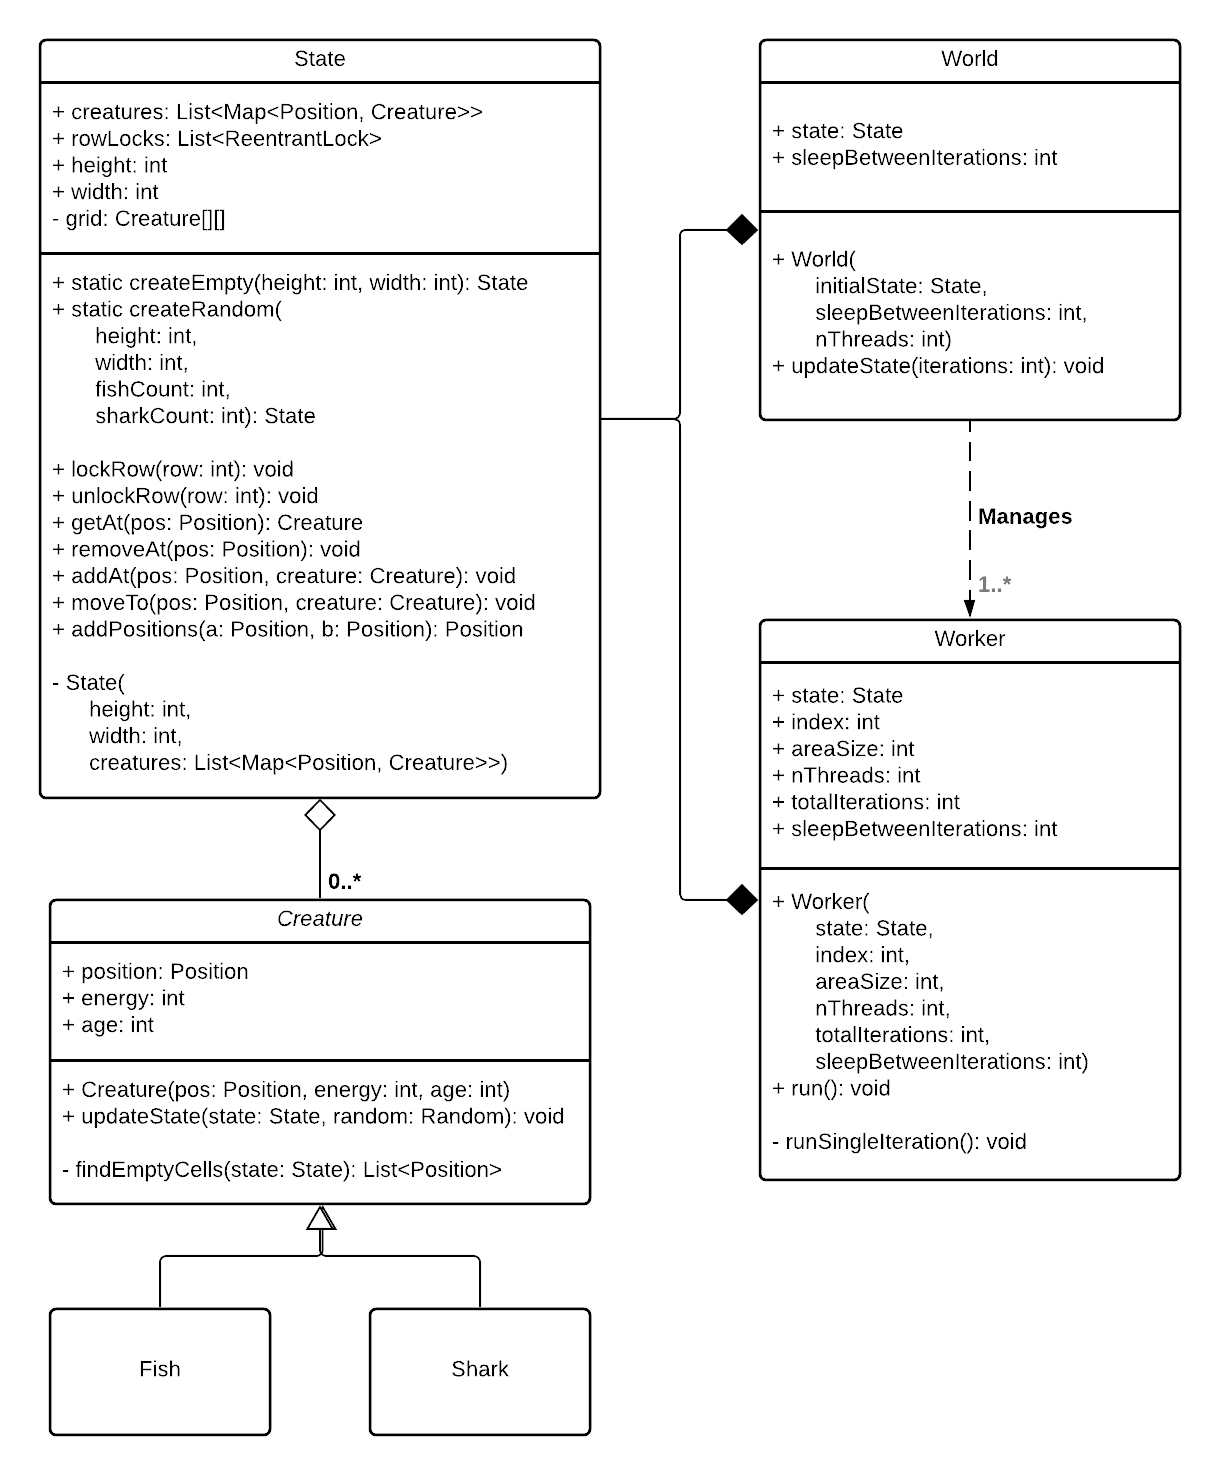
\includegraphics[width=1.1\textwidth]{classes-uml.png}
	\caption{UML Клас диаграма на проекта}
	\label{fig:figure1}
\end{figure}

\section{Тестови резултати}

\section{Бъдещо развитие на проекта}
Използване на Dynamic domain decomposition

\begin{figure}[H]
	\centering
	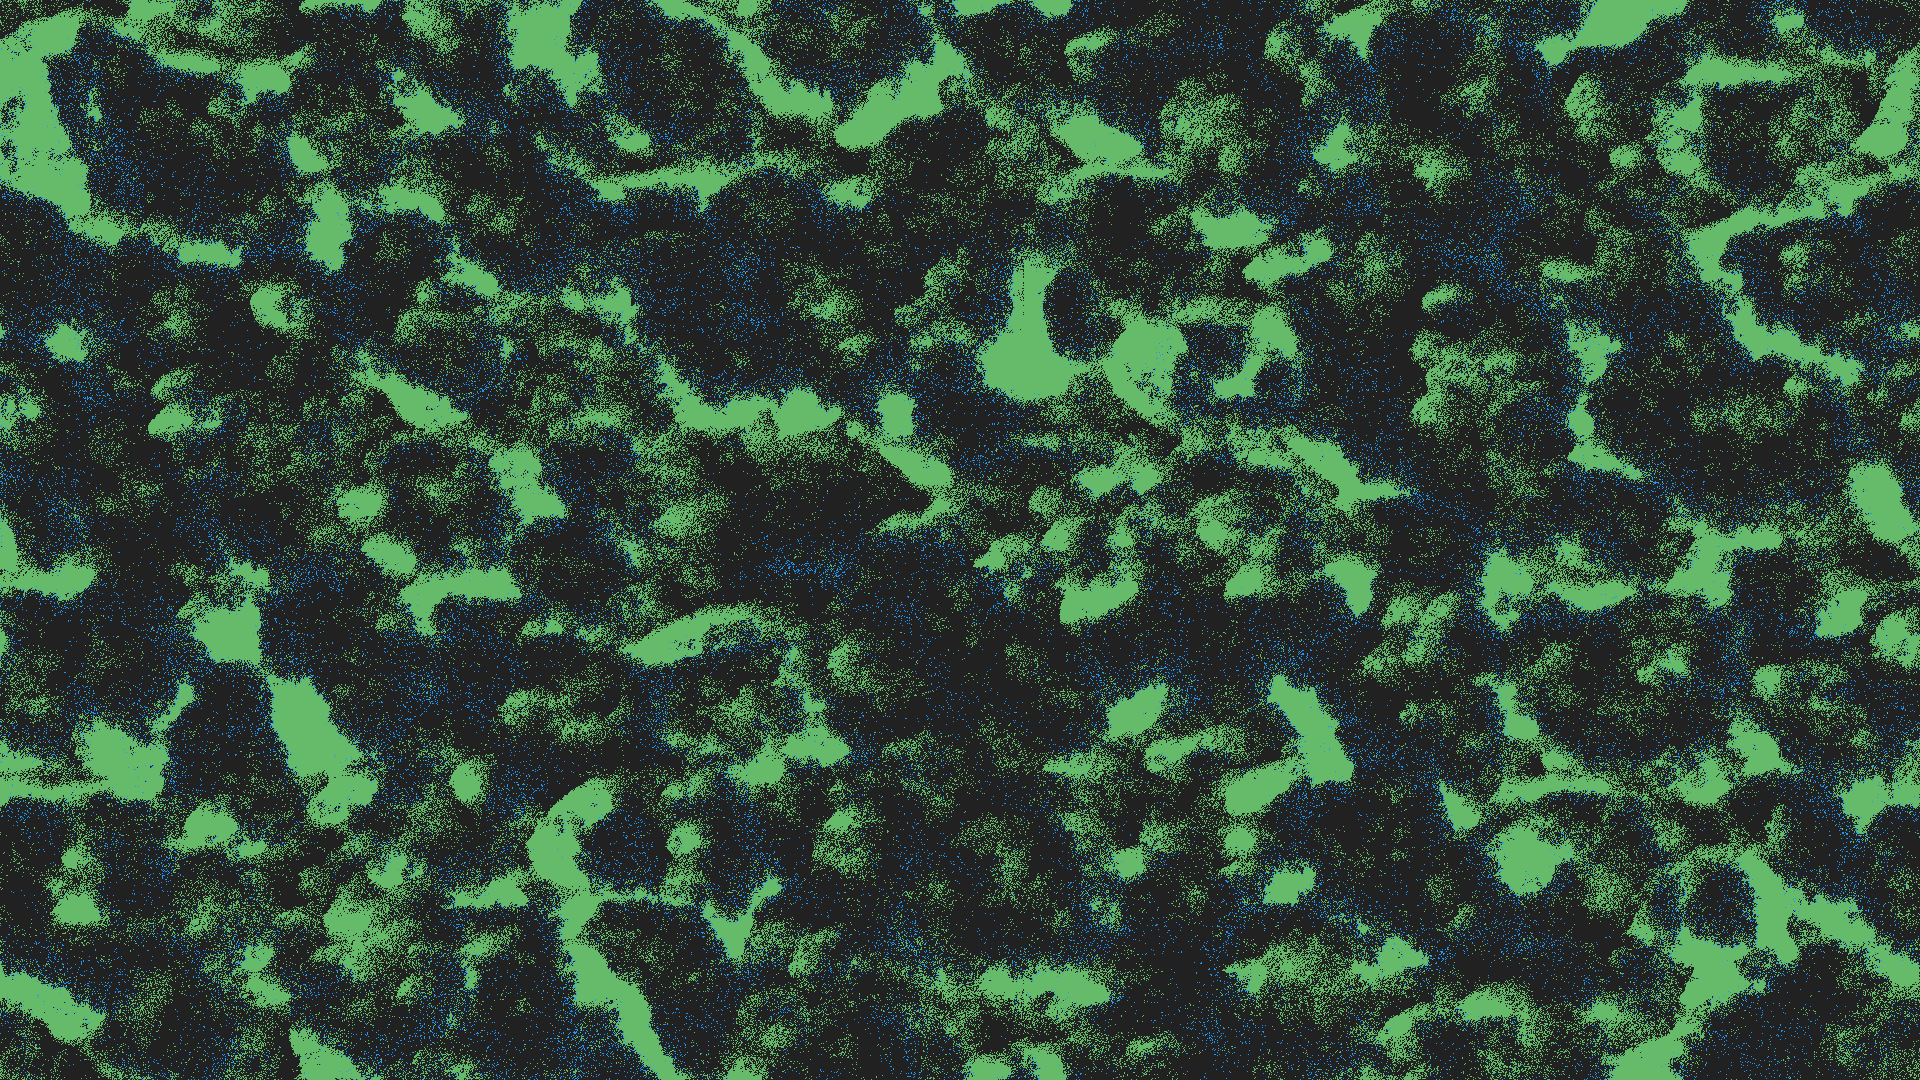
\includegraphics[width=1\textwidth]{screenshot-big.png}
	\caption{Симулацията със размер на полето 1920x1080, 1 000 000 херинги и 100 000 акули}
	\label{fig:figure2}
\end{figure}

\begin{figure}[H]
	\centering
	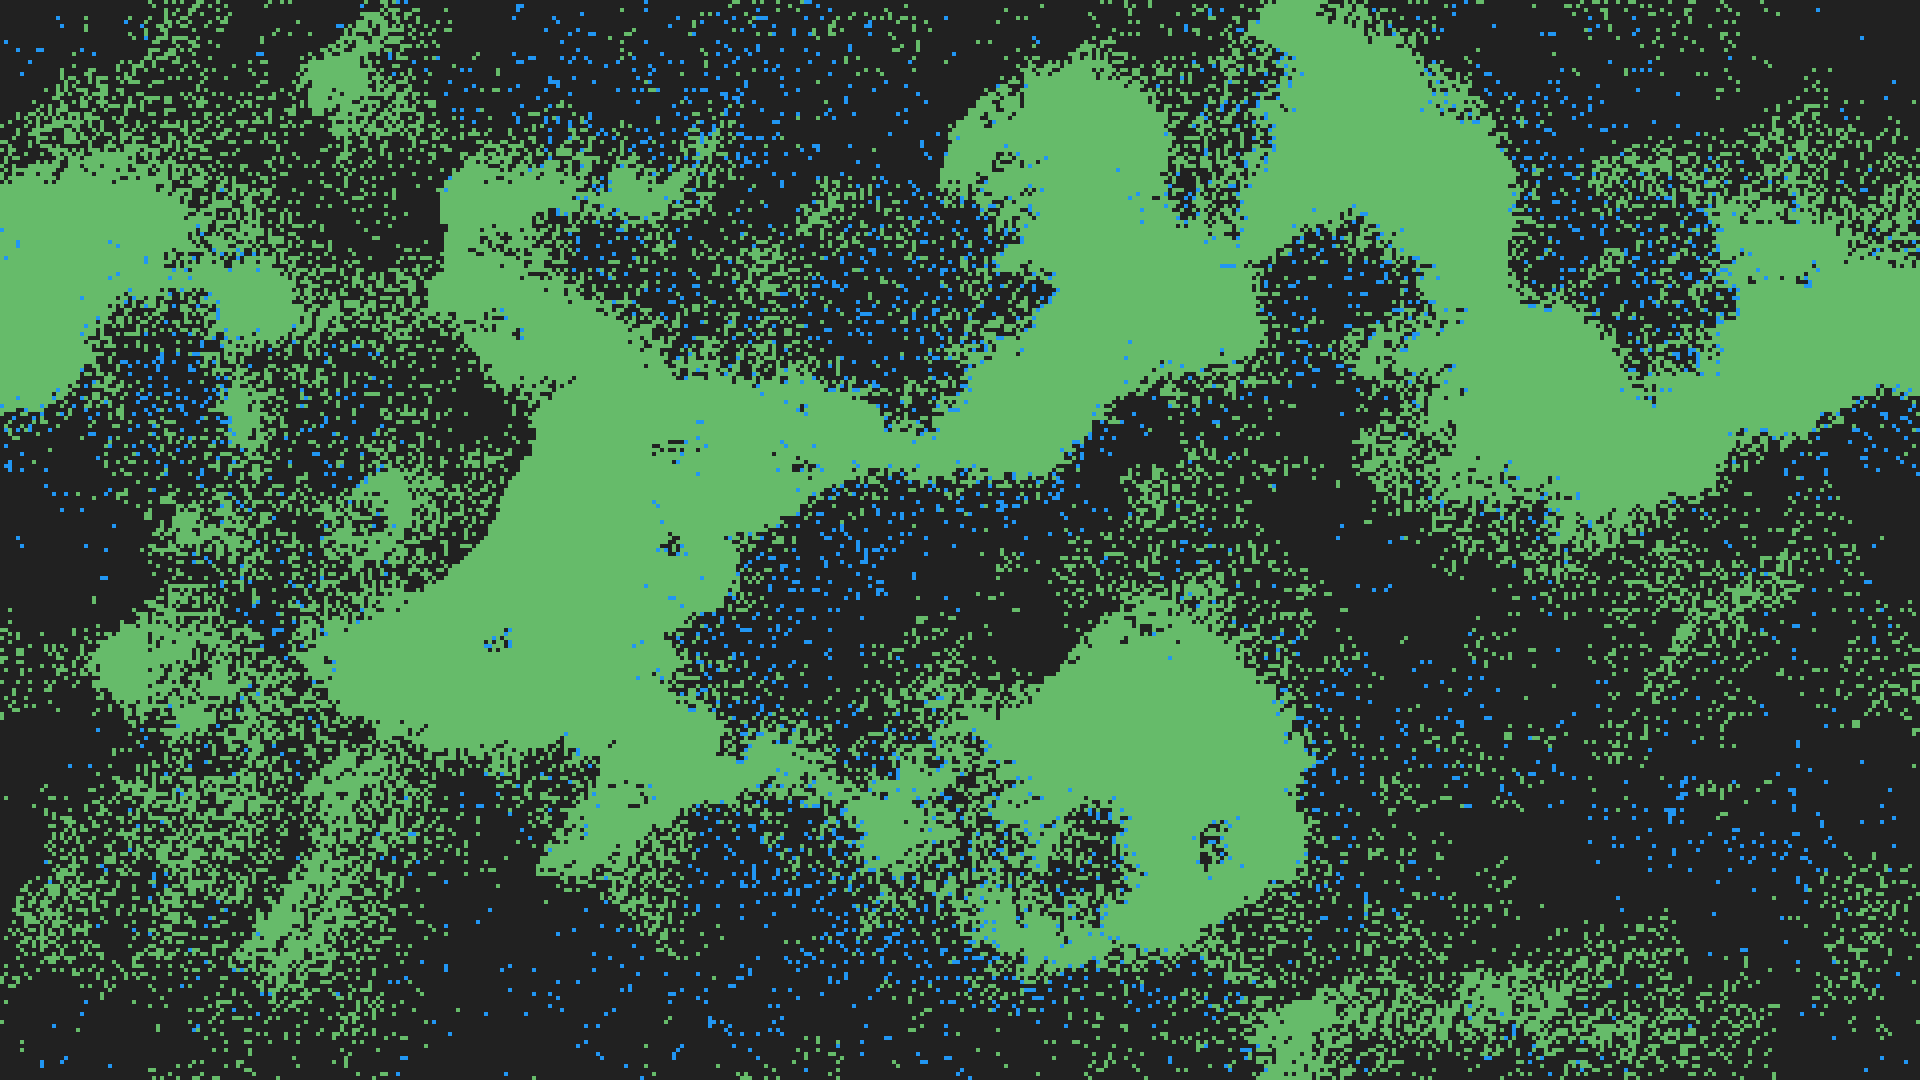
\includegraphics[width=1\textwidth]{screenshot-small.png}
	\caption{Симулацията със размер на полето 480x270, 10 000 херинги и 1000 хиляди акули}
	\label{fig:figure3}
\end{figure}

\bibliography{wator}{}
\bibliographystyle{plain}
\end{document}
